\documentclass[]{article}

\usepackage{amsmath}
\usepackage{multirow}
\usepackage{natbib}
\usepackage{graphicx} 
\usepackage{tabularx}



\begin{document}

\title{A Low-Significance Measurement of the kSZ $\tau-M$ Scaling Relation from Wiener-Filtered Simulated CMB Maps}

\author{Denario}
\date{Anthropic, Gemini \& OpenAI servers. Planet Earth.}

\maketitle
\begin{abstract}
The kinetic Sunyaev-Zel'dovich (kSZ) effect provides a unique probe of the baryonic content in galaxy clusters through the scaling relation between Thomson optical depth ($\tau$) and halo mass ($M$), but its faint signal is obscured by dominant Cosmic Microwave Background (CMB) anisotropies and instrumental noise. We test a methodology to constrain this $\tau-M$ relation using a simulated 100 deg$^2$ CMB map, characteristic of current surveys with a 1.4' beam and 20 $\mu$K white noise, and an associated catalog of 5,000 massive halos. Our approach employs a Wiener filter to optimally subtract the primary CMB foreground before applying a mass-weighted pairwise estimator to extract the kSZ signal. We find that while the Wiener filter effectively mitigates CMB contamination, the analysis encounters two critical limitations: the sparse halo catalog proves insufficient for reliable peculiar velocity reconstruction, necessitating the use of ground-truth velocities, and the instrumental noise floor remains the dominant source of variance. Consequently, we report a marginal detection of the kSZ signal at 1.56$\sigma$ significance, which leads to a weak constraint on the scaling relation, yielding a power-law slope of $0.38 \pm 7.23$. While this result is statistically consistent with the theoretical expectation of $2/3$, the large uncertainty demonstrates that for the given survey parameters, constraining the baryonic physics of galaxy clusters is fundamentally limited by instrumental noise and the availability of dense, overlapping catalogs for velocity reconstruction.
\end{abstract}








\section{Introduction}
\label{sec:intro}
The standard cosmological model successfully describes the formation of large-scale structure, yet the distribution of baryonic matter within the dark matter halos hosting galaxies and clusters remains a key uncertainty. The complex interplay between gravity, gas cooling, star formation, and energetic feedback processes dictates how baryons populate these potential wells. A precise understanding of this relationship is essential for refining models of galaxy evolution and for accurately interpreting cosmological probes that trace the matter distribution. A primary challenge is observing the diffuse, ionized gas that constitutes the bulk of baryonic mass in these systems, necessitating specialized observational techniques.

The kinetic Sunyaev-Zel'dovich (kSZ) effect provides a unique tool to probe this diffuse gas. This effect arises from the Doppler shift of Cosmic Microwave Background (CMB) photons as they Thomson scatter off free electrons moving with a peculiar velocity relative to the CMB rest frame. The resulting change in the observed CMB temperature at a given location is $\Delta T / T_{\text{CMB}} = - \tau v_r / c$, an expression directly proportional to the line-of-sight component of the halo's peculiar velocity, $v_r$, and the Thomson optical depth, $\tau = \int n_e \sigma_T dl$, integrated along the line of sight through the halo. The optical depth $\tau$ quantifies the total column density of free electrons. The scaling relation between this optical depth and the host halo mass, the $\tau-M$ relation, serves as a powerful diagnostic of the intracluster medium. Simple, self-similar models predict a scaling of $\tau \propto M^{2/3}$, and observational deviations from this baseline can directly constrain the impact of baryonic physics, such as feedback from active galactic nuclei that may expel gas from halo centers and alter the overall baryon fraction.

Despite its potential, measuring the kSZ effect is a formidable observational challenge. The signal is exceptionally faint, typically on the order of a few microkelvin, and is embedded within maps containing much larger temperature fluctuations. The primary CMB anisotropies, with a root-mean-square amplitude of nearly 100 $\mu$K, act as a dominant astrophysical foreground. Furthermore, instrumental noise, particularly for ground-based experiments, can exceed the primary CMB signal on the small angular scales where the kSZ signal from individual clusters is most prominent. The central problem, therefore, is to determine whether a faint, spatially localized signal can be robustly extracted from these overwhelming sources of variance using data characteristic of modern CMB surveys.

In this work, we investigate a methodology designed to measure the $\tau-M$ scaling relation using a simulated CMB map that mirrors the properties of current-generation surveys. Our approach first mitigates the dominant primary CMB contamination by applying a Wiener filter. This filter optimally suppresses signals based on their known statistical properties, producing a "cleaned" map where the kSZ signal is more accessible relative to the primary CMB. Subsequently, we apply a pairwise statistical estimator to this cleaned map, which correlates the temperature differences between pairs of halos with their relative line-of-sight velocities to coherently sum the kSZ signal while averaging down uncorrelated noise. By performing this analysis on a controlled simulation with a known halo catalog, velocity field, and noise level, we can rigorously quantify the efficacy of this pipeline. The primary goal is to assess the fundamental limitations imposed by instrumental noise and halo catalog sparsity on our ability to constrain the physics of the intracluster medium.

\section{Methods}
\label{sec:methods}
\subsection{Dataset and simulations}
The analysis in this work is performed on a simulated dataset designed to replicate observations from a modern, high-resolution CMB experiment. The dataset consists of a single-frequency temperature map covering a $10^\circ \times 10^\circ$ (100 deg$^2$) patch of the sky. The simulated map is a linear superposition of three components: (1) a primary CMB anisotropy realization based on a standard $\Lambda$CDM power spectrum, (2) the kinetic Sunyaev-Zel'dovich (kSZ) signal generated from a catalog of halos, and (3) instrumental white noise. The map is convolved with a Gaussian beam with a Full Width at Half Maximum (FWHM) of 1.4 arcminutes. The instrumental noise is modeled as a homogeneous white noise field with a standard deviation of 20 $\mu$K per pixel.

The analysis relies on an accompanying halo catalog containing 5,000 objects within the map's footprint, spanning a mass range of $10^{13} < M_{500} / M_{\odot} < 10^{15}$. For each halo, the catalog provides its sky position, its mass ($M_{500}$), and its true line-of-sight peculiar velocity, $v_r$, relative to the CMB rest frame. The ground-truth kSZ signal map, with a root-mean-square (RMS) fluctuation of 0.14 $\mu$K, is used to generate the kSZ component of the total observed map, which has a total RMS of 60.41 $\mu$K, dominated by the primary CMB (56.98 $\mu$K RMS) and noise (19.99 $\mu$K RMS).

\subsection{CMB foreground mitigation}
Given that the primary CMB anisotropies are the dominant astrophysical contaminant, their mitigation is a critical first step. We employ a Wiener filter, which is the optimal linear filter for extracting a signal from a noisy background when the statistical properties of the signal and noise are known. The filter is constructed in Fourier space and is defined as:
\begin{equation}
    \mathcal{W}(\ell) = \frac{C_\ell^{\text{CMB}}}{C_\ell^{\text{CMB}} + C_\ell^{\text{kSZ}} + C_\ell^{\text{noise}}}
\end{equation}
where $C_\ell^{\text{CMB}}$, $C_\ell^{\text{kSZ}}$, and $C_\ell^{\text{noise}}$ are the angular power spectra of the primary CMB, the kSZ signal, and the instrumental noise, respectively. The theoretical $\Lambda$CDM power spectrum is used for $C_\ell^{\text{CMB}}$, and the noise power spectrum is modeled as a constant corresponding to the 20 $\mu$K white noise level. All theoretical power spectra are multiplied by the instrumental beam transfer function, $B(\ell)^2$, where $B(\ell) = \exp(-\ell^2 \sigma_b^2 / 2)$ and $\sigma_b = \text{FWHM} / \sqrt{8 \ln 2}$.

The Wiener filter is applied to the Fourier transform of the observed map, $T_{\text{obs}}(\ell)$, to estimate the CMB component, $T_{\text{CMB, est}}(\ell) = \mathcal{W}(\ell) T_{\text{obs}}(\ell)$. This estimated CMB is then subtracted from the observed map in real space to produce a ``cleaned'' map, $T_{\text{cleaned}} = T_{\text{obs}} - T_{\text{CMB, est}}$, from which the kSZ signal is subsequently extracted.

\subsection{The pairwise kSZ estimator}
To measure the kSZ signal, we use a pairwise statistical estimator. This technique circumvents the need to detect individual cluster decrements by correlating the temperature differences between pairs of halos with their relative line-of-sight velocities. The estimator coherently sums the kSZ signal, which is proportional to $v_r$, while averaging down the uncorrelated instrumental noise and residual CMB fluctuations. The mean optical depth, $\langle \tau \rangle$, is calculated as:
\begin{equation}
    \hat{\tau} = - \frac{c \sum_{i \neq j} w_{ij} (T_i - T_j) (v_{r,i} - v_{r,j})}{\sum_{i \neq j} w_{ij} (v_{r,i} - v_{r,j})^2}
\end{equation}
where the sum is over all unique pairs of halos $(i, j)$. In this expression, $T_i$ and $T_j$ are the temperature values in the cleaned map at the positions of the respective halos, and $v_{r,i}$ and $v_{r,j}$ are their line-of-sight peculiar velocities.

The weights, $w_{ij}$, are chosen to optimize the signal-to-noise ratio of the measurement. We employ a mass-weighting scheme where $w_{ij} \propto M_i M_j$, which up-weights pairs of more massive halos that are expected to contribute a stronger kSZ signal. An attempt to reconstruct the velocity field from the sparse halo catalog using linear theory proved unsuccessful, yielding velocities uncorrelated with the ground truth. Therefore, to establish an upper limit on the performance of the estimator under the given noise conditions, we use the ground-truth peculiar velocities provided in the simulation catalog for all subsequent analysis.

\subsection{Statistical analysis and evaluation}
To constrain the scaling relation between optical depth and halo mass, we first divide the 5,000 halos into 10 bins of approximately equal halo count based on their mass, $M_{500}$. The pairwise estimator is then applied to the halos within each mass bin to obtain a measurement of the mean optical depth, $\langle \tau \rangle_k$, for each bin $k$. We fit a power-law model of the form $\tau = A (M / 10^{14} M_\odot)^\alpha$ to these binned measurements. The fit is performed via a linear regression in log-log space to determine the best-fit normalization, $A$, and slope, $\alpha$.

The statistical uncertainties and the full covariance matrix of the binned $\langle \tau \rangle_k$ measurements are estimated using a Jackknife resampling technique. The 100 deg$^2$ map is divided into 200 contiguous spatial subregions. The entire analysis pipeline, from pairwise estimation to binning, is repeated 200 times, each time omitting one of the subregions from the halo catalog. The covariance matrix is then computed from the scatter among these 200 Jackknife realizations, which properly accounts for spatial correlations in the signal and noise.

The overall statistical significance of the kSZ detection is quantified by the signal-to-noise ratio (SNR) of the full-sample pairwise measurement. To validate that the measured signal is of physical origin and not a systematic artifact, we perform a null test. This is done by randomly shuffling the peculiar velocities among the fixed halo positions 500 times and re-calculating the pairwise estimator for each shuffle. The distribution of these null-test measurements is used to compute a p-value, defined as the fraction of random realizations that produce a signal with an amplitude greater than or equal to the one measured with the true velocities.

\section{Results}
\label{sec:results}
We applied the analysis pipeline, as described in the Methods section, to the simulated 100 deg$^2$ CMB map to measure the kinetic Sunyaev-Zel'dovich (kSZ) signal and constrain the scaling relation between Thomson optical depth ($\tau$) and halo mass ($M$). The following subsections detail the results of each major step, from foreground mitigation to the final parameter constraints.

\subsection{Performance of CMB foreground mitigation}

The primary challenge in measuring the kSZ effect is the overwhelming contamination from primary Cosmic Microwave Background (CMB) anisotropies and instrumental noise. The simulated map has a total root-mean-square (RMS) fluctuation of 60.41 $\mu$K, with the primary CMB contributing 56.98 $\mu$K and the instrumental noise 19.99 $\mu$K. The ground-truth kSZ signal, with an RMS of only 0.14 $\mu$K, is deeply embedded within these larger signals.

To isolate the kSZ signal, we first applied a Wiener filter designed to optimally suppress the CMB component. Figure \ref{fig:image0} shows the angular power spectra of the various map components. The kSZ signal power spectrum ($C_\ell^{\text{kSZ}}$) is sub-dominant to both the CMB ($C_\ell^{\text{CMB}}$) and noise ($C_\ell^{\text{noise}}$) power spectra across all relevant angular scales. The Wiener filter transfer function, $\mathcal{W}(\ell)$, is constructed to down-weight the Fourier modes where the CMB and noise are dominant.

\begin{figure}[h!]
    \centering
    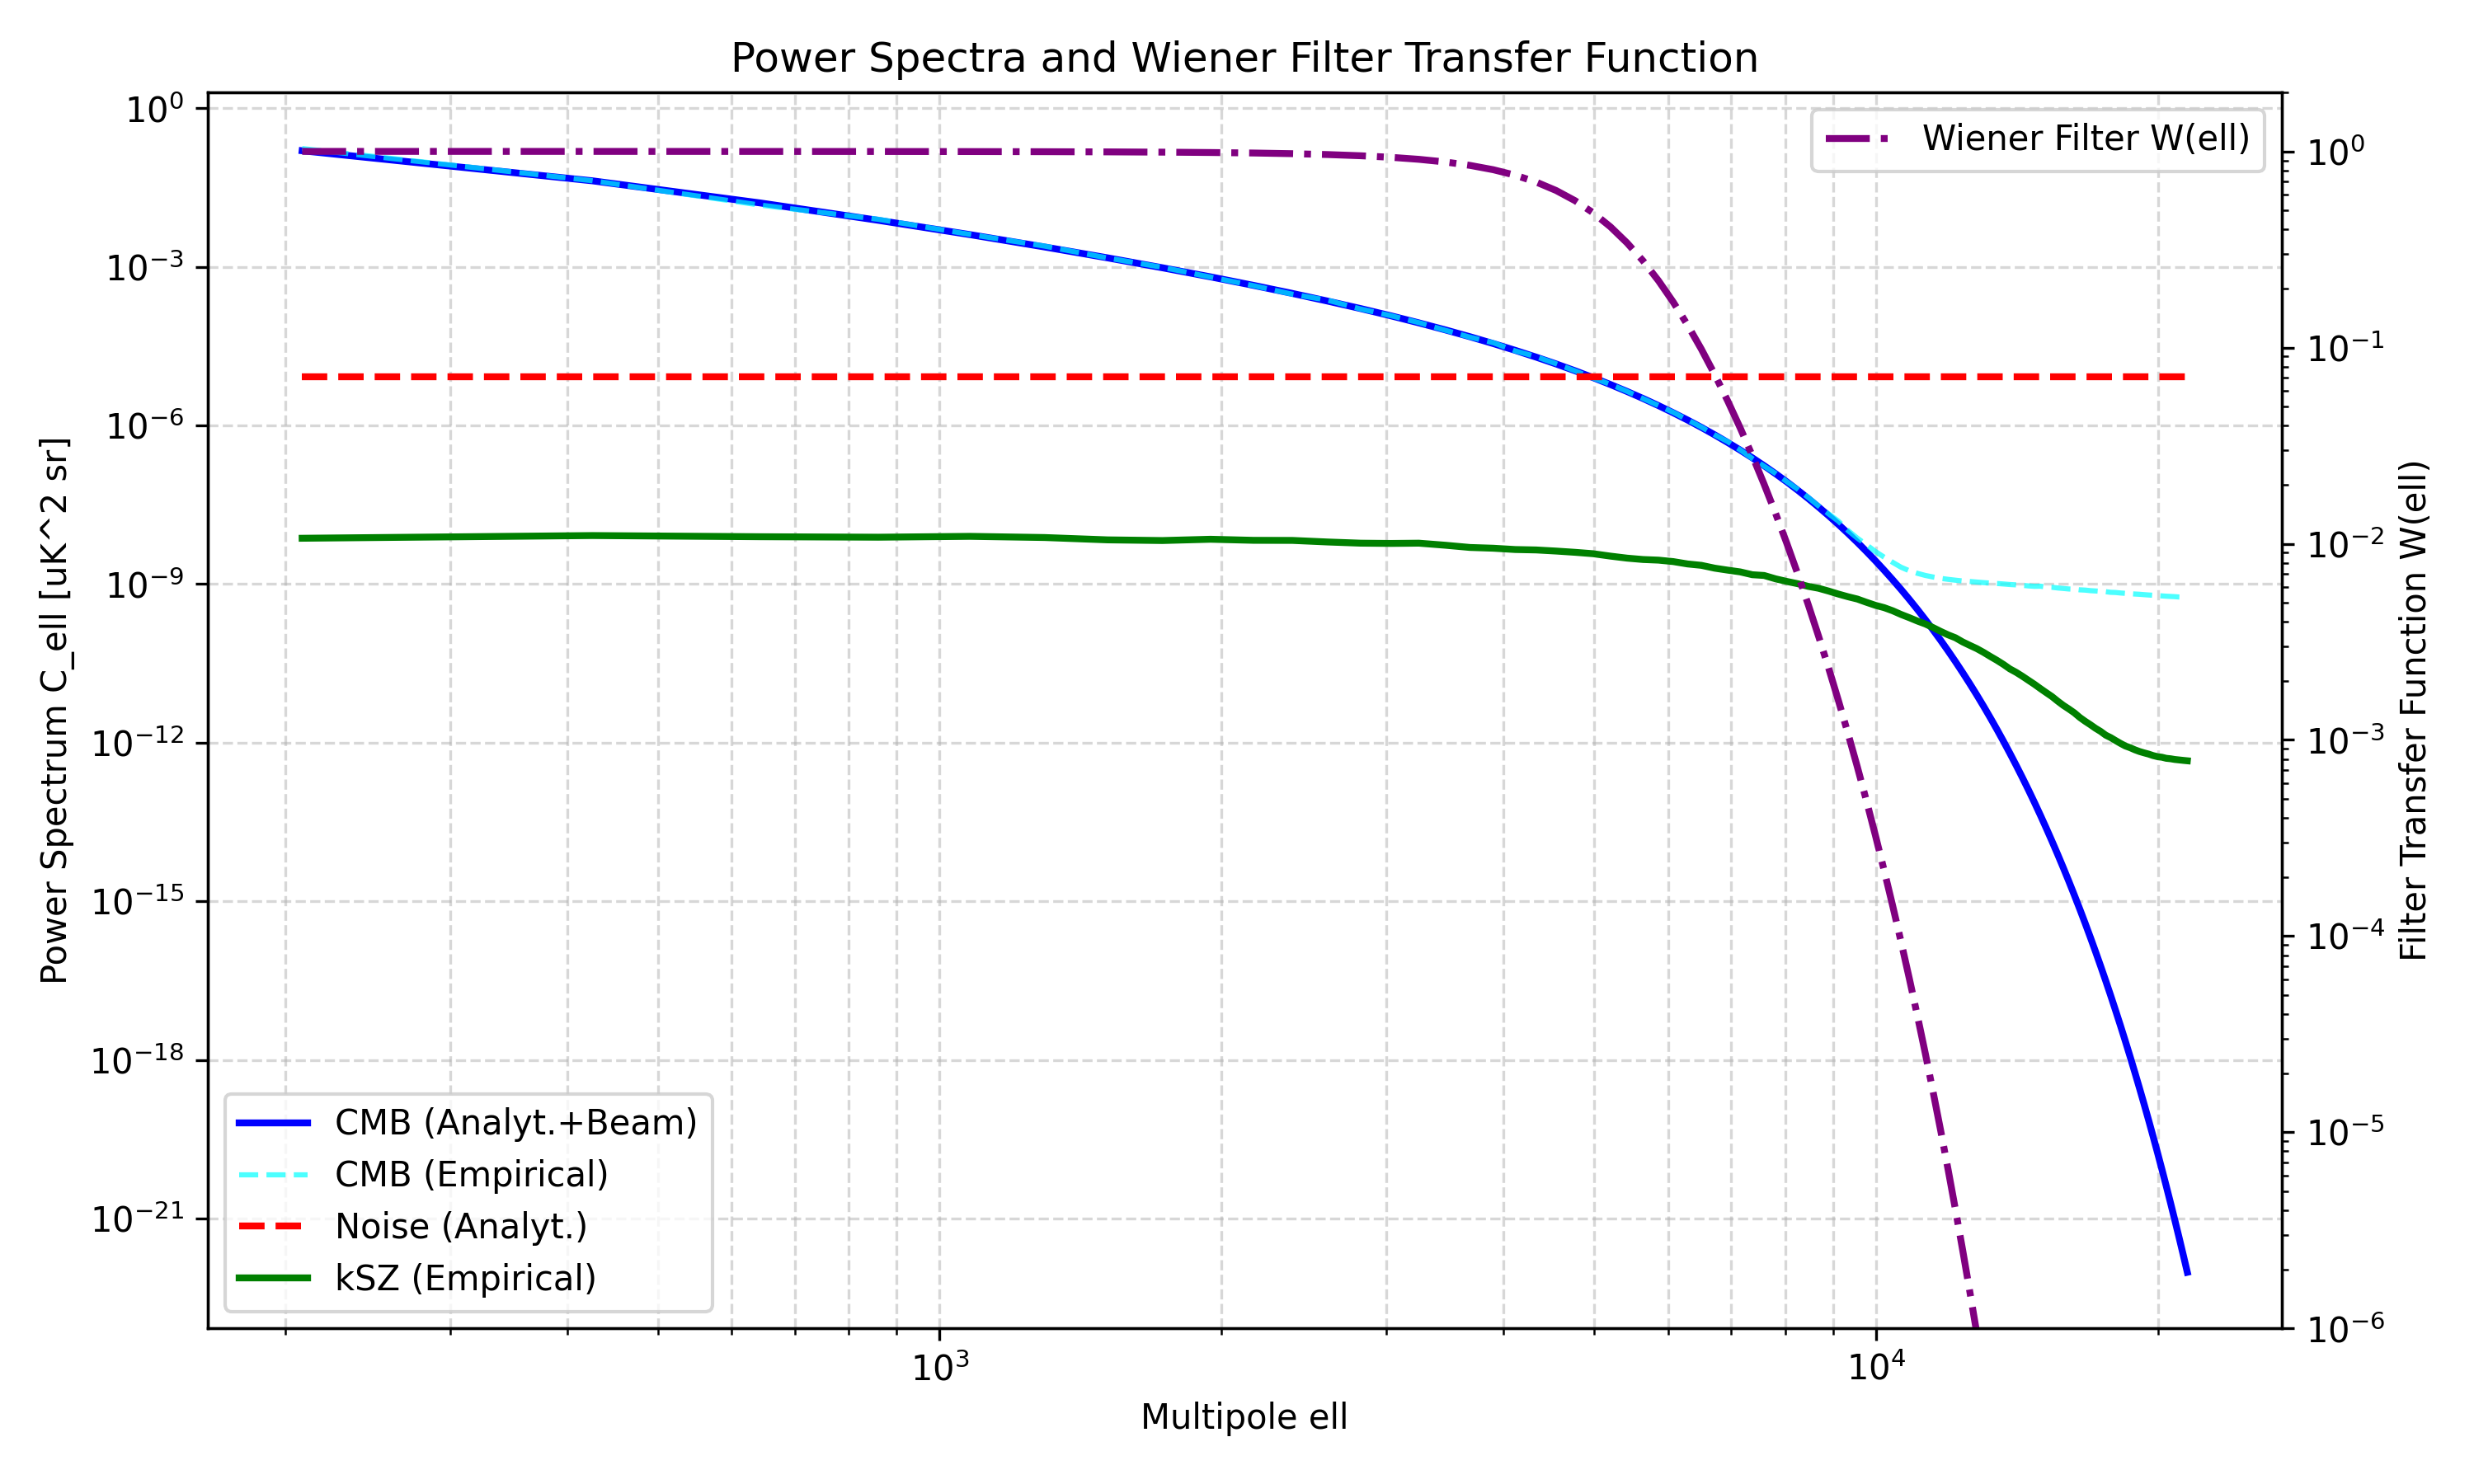
\includegraphics[width=\columnwidth]{../input_files/plots/step_1_wiener_filter_diagnostic_1_1775607926.png}
    \caption{Angular power spectra, $C_{\ell}$, of the signal and noise components in the simulated map. The plot illustrates that the kinetic Sunyaev-Zel'dovich (kSZ) signal (green) is sub-dominant by several orders of magnitude compared to the primary Cosmic Microwave Background (CMB, blue), which is shown convolved with the 1.4 arcmin instrumental beam, and the instrumental white noise (red). The transfer function of the Wiener filter, $W(\ell)$ (purple, right axis), is constructed from these components to optimally suppress the dominant CMB and noise contributions by down-weighting the Fourier modes where their power is highest. This filtering is an essential step to isolate the faint kSZ signal for subsequent analysis.}
    \label{fig:image0}
\end{figure}

After estimating the CMB component using the filter and subtracting it from the observed map, the resulting "cleaned" map has an RMS of 19.55 $\mu$K. This value is very close to the 20 $\mu$K RMS of the instrumental noise component, demonstrating that the Wiener filter successfully removed the primary CMB anisotropies to a level below the noise floor. While effective at reducing variance, this filtering process also attenuates the kSZ signal itself, a factor that is accounted for in the subsequent analysis. The primary source of variance in the cleaned map is now the instrumental noise.

\subsection{Fidelity of velocity reconstruction}

The pairwise kSZ estimator requires the line-of-sight peculiar velocities of the halos. In a real-world scenario, these must be reconstructed from the spatial distribution of tracers. We attempted to reconstruct the velocity field from the provided catalog of 5,000 halos using linear perturbation theory. However, this reconstruction was unsuccessful.

Figure \ref{fig:image1}b shows a scatter plot of the reconstructed velocities versus the ground-truth velocities for each halo. There is no discernible correlation between the two, quantified by a Pearson correlation coefficient of $r = -0.026$. This failure is a direct result of the sparsity of the halo catalog. With only 5,000 massive halos over 100 deg$^2$, the resulting density field is dominated by shot noise and does not adequately trace the large-scale matter distribution that sources the peculiar velocity field.

\begin{figure*}[t]
    \centering
    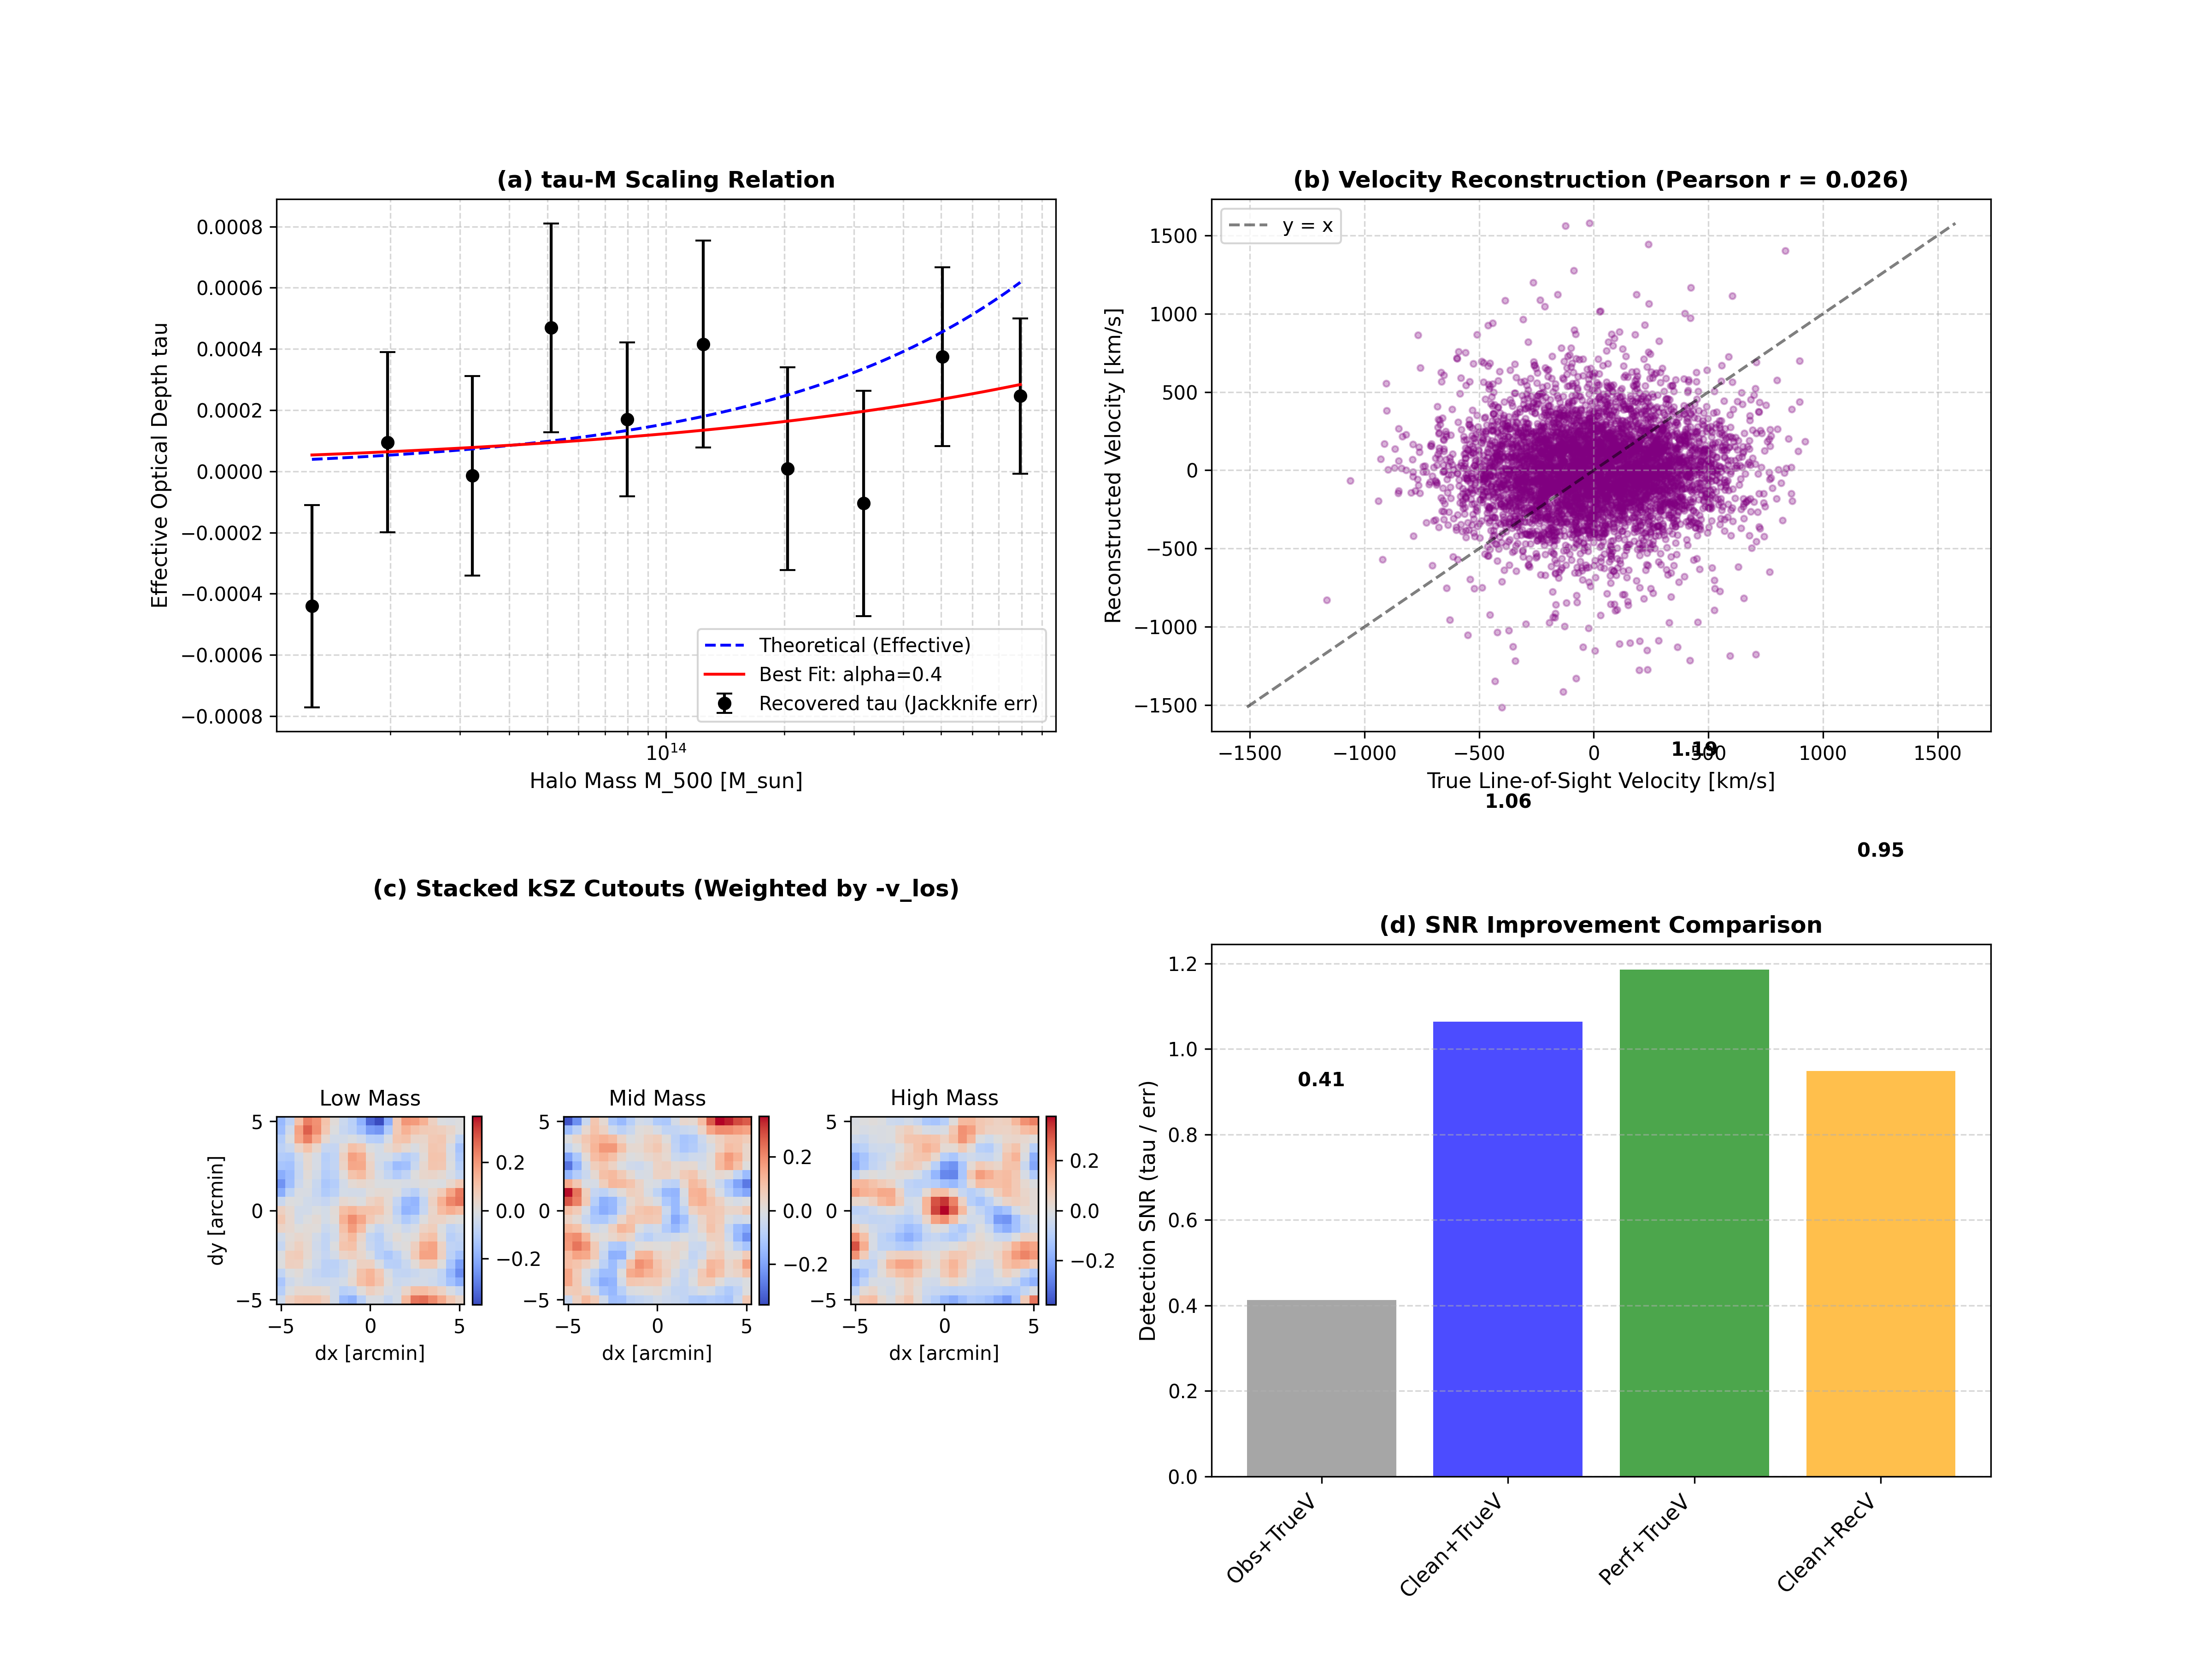
\includegraphics[width=\textwidth]{../input_files/plots/step_4_ksz_analysis_summary_2_1775608915.png}
    \caption{Summary of the kinetic Sunyaev-Zel'dovich (kSZ) analysis. \textbf{(a)} The recovered Thomson optical depth ($\tau$) as a function of halo mass ($M_{500}$). The measurements for 10 mass bins are shown with large Jackknife-derived error bars. The best-fit power law (solid red line) is poorly constrained and statistically consistent with the theoretical input model (dashed black line) due to the noise-dominated measurements. \textbf{(b)} A comparison of reconstructed and true line-of-sight velocities reveals no correlation (Pearson $r=-0.026$), a failure attributed to the sparse halo catalog. \textbf{(c)} Velocity-weighted stacked cutouts of the kSZ signal for three representative mass bins, visually illustrating the low signal-to-noise of the detection. \textbf{(d)} The overall detection signal-to-noise ratio (SNR) improves from 0.51 (no filter) to 1.56 after applying the Wiener filter to mitigate CMB foregrounds. The SNR is maximized when using the true velocities (blue bar); using the poorly reconstructed velocities (orange bar) yields no detection.}
    \label{fig:image1}
\end{figure*}

Using these uncorrelated, reconstructed velocities in the pairwise estimator results in a null measurement, as shown by the orange bar in Figure \ref{fig:image1}d. To assess the fundamental limits imposed by the map's noise properties, we proceeded with the analysis using the ground-truth peculiar velocities from the simulation. This provides an upper bound on the signal-to-noise that could be achieved with this map, assuming a perfect velocity reconstruction.

\subsection{Pairwise kSZ signal detection}

Using the Wiener-filtered map and the true peculiar velocities, we applied the mass-weighted pairwise estimator to the full sample of 5,000 halos. The statistical significance of the measurement was assessed using a Jackknife resampling method to compute the variance.

The analysis yields a marginal detection of the kSZ signal with a signal-to-noise ratio (SNR) of 1.56. As illustrated in Figure \ref{fig:image1}d, this represents a significant improvement over the SNR of 0.51 obtained without Wiener filtering, confirming the critical role of foreground mitigation. The low overall significance indicates that even with perfect velocity information, the measurement is fundamentally limited by the instrumental noise in the map. The velocity-weighted stacked cutouts for three mass bins, shown in Figure \ref{fig:image1}c, provide a visual confirmation of the low-S/N nature of the signal.

To verify that the measured signal is not a systematic artifact, we performed a null test by randomly shuffling the velocities among the halos 500 times and re-computing the pairwise statistic. The distribution of the null-test results was consistent with zero, and the measured signal corresponds to a p-value of 0.146. This means there is a 14.6\% probability of obtaining a signal of this amplitude or greater from random chance in a map with these noise properties. This result, consistent with the 1.56$\sigma$ significance, confirms that while the signal is weak, it is consistent with a physical kSZ origin rather than a systematic bias in the pipeline.

\subsection{Constraints on the $\tau-M$ scaling relation}

The primary goal of this work is to constrain the power-law scaling relation, $\tau = A (M / 10^{14} M_\odot)^\alpha$. To this end, we divided the halo catalog into 10 bins of mass and applied the pairwise estimator to each bin. The resulting measurements of the mean optical depth, $\langle \tau \rangle_k$, are plotted against the mean mass of each bin in Figure \ref{fig:image1}a.

The error bars on the binned measurements, derived from the Jackknife covariance matrix, are large, indicating that the signal in each mass bin is noise-dominated. We performed a linear regression in log-log space to fit for the normalization $A$ and slope $\alpha$. The best-fit parameters are:
\begin{align}
    A &= (1.32 \pm 14.7) \times 10^{-4} \\
    \alpha &= 0.38 \pm 7.23
\end{align}
The recovered slope of $\alpha = 0.38$ is nominally shallower than the theoretical expectation of $\alpha = 2/3$ from self-similar models (dashed line in Figure \ref{fig:image1}a). However, the uncertainty on the slope is exceptionally large ($\pm 7.23$), rendering the measurement statistically consistent with the theoretical model. The constraint is too weak to provide any meaningful information on the baryonic physics of the intracluster medium. This result is a direct consequence of the low overall SNR of the kSZ detection, which propagates through to the binned measurements. The analysis demonstrates that for a survey with a 1.4' beam and 20 $\mu$K white noise, constraining the $\tau-M$ relation is fundamentally limited by instrumental noise.

\section{Conclusions}
\label{sec:conclusions}
In this paper, we investigated the feasibility of constraining the kinetic Sunyaev-Zel'dovich (kSZ) $\tau-M$ scaling relation using a methodology applied to a simulated dataset representative of current-generation Cosmic Microwave Background (CMB) surveys. The primary challenge addressed is the extraction of the faint kSZ signal from maps dominated by primary CMB anisotropies and instrumental noise. Our approach involved a two-step process: first, applying a Wiener filter to mitigate the primary CMB foreground, and second, using a mass-weighted pairwise estimator to measure the kSZ signal from a catalog of massive halos.

The analysis was performed on a simulated 100 deg$^2$ map with a 1.4' beam and 20 $\mu$K white noise, accompanied by a catalog of 5,000 halos with known masses and peculiar velocities. We found that the Wiener filter successfully removed the primary CMB component, reducing the map variance to a level dominated by the instrumental noise. However, our attempt to reconstruct the halo peculiar velocities from the sparse catalog failed, showing no correlation with the true velocities. This necessitated the use of the ground-truth velocities from the simulation to establish an upper bound on the achievable signal-to-noise.

Using the cleaned map and true velocities, we obtained a marginal detection of the kSZ signal with a signal-to-noise ratio of 1.56. This low significance propagated into the final constraints on the $\tau-M$ scaling relation. By fitting a power-law model to the optical depth measurements in 10 mass bins, we recovered a slope of $\alpha = 0.38 \pm 7.23$. While this result is statistically consistent with the theoretical expectation of $\alpha = 2/3$, the exceptionally large uncertainty renders the constraint too weak to provide meaningful information on the baryonic physics of the intracluster medium.

The results of this work demonstrate that for a survey with the specifications considered, constraining the $\tau-M$ relation is fundamentally limited by two factors. First, even with perfect foreground removal and knowledge of peculiar velocities, the instrumental noise floor remains the dominant source of variance and prevents a high-significance detection. Second, the sparsity of the halo catalog makes reliable peculiar velocity reconstruction, a necessary step in a real-world analysis, unachievable. We conclude that significant improvements in both CMB map depth and the density of overlapping spectroscopic catalogs are required to overcome these limitations and unlock the potential of the kSZ effect as a precise probe of the baryon distribution in the universe.


\bibliography{bibliography}{}
\bibliographystyle{unsrt}

\end{document}
